\documentclass[11pt]{article}
\usepackage[a4paper,margin=23mm]{geometry}
\usepackage{amsmath,amssymb,amsthm,mathtools}
\usepackage{graphicx}
\usepackage{microtype}
\usepackage{xcolor}
\usepackage[colorlinks=true,linkcolor=blue!55!black,citecolor=blue!55!black,urlcolor=blue!55!black]{hyperref}

\newtheorem{theorem}{Theorem}
\newtheorem{lemma}[theorem]{Lemma}
\newtheorem{proposition}[theorem]{Proposition}
\newtheorem{corollary}[theorem]{Corollary}
\theoremstyle{definition}
\newtheorem{definition}[theorem]{Definition}
\newcommand{\lipf}{\operatorname{lip}}
\newcommand{\Lipf}{\operatorname{Lip}}
\newcommand{\LLip}{\mathbb L\!\operatorname{ip}}
\newcommand{\R}{\mathbb R}
\newcommand{\len}{\operatorname{length}}

\title{Lipschitz-Derivative Triples Beyond Convex Domains\\
\large A locally length-space theorem and two sharp obstructions}
\author{Candidate partial result for arXiv:2509.20849}
\date{13 August 2026}

\begin{document}
\maketitle

\begin{center}
\fbox{\parbox{0.92\linewidth}{\textbf{Status: candidate substantial partial proof, likely valid.}
The packet extends the source's strongest joint necessary condition from
locally convex normed domains to locally length metric spaces, proves a
quantitative quasiconvex version, and shows both that the source's necessary
conditions are not sufficient and that the Baire identity fails on general
compact connected metric subspaces.  It does not classify all realizable
triples.  Novelty remains subject to expert literature review.}}
\end{center}

\section{Source question and scope}

Maslyuchenko and W\'ojcicki ask the following inverse problem on source PDF
p.~2 \cite{MW}:

\begin{center}
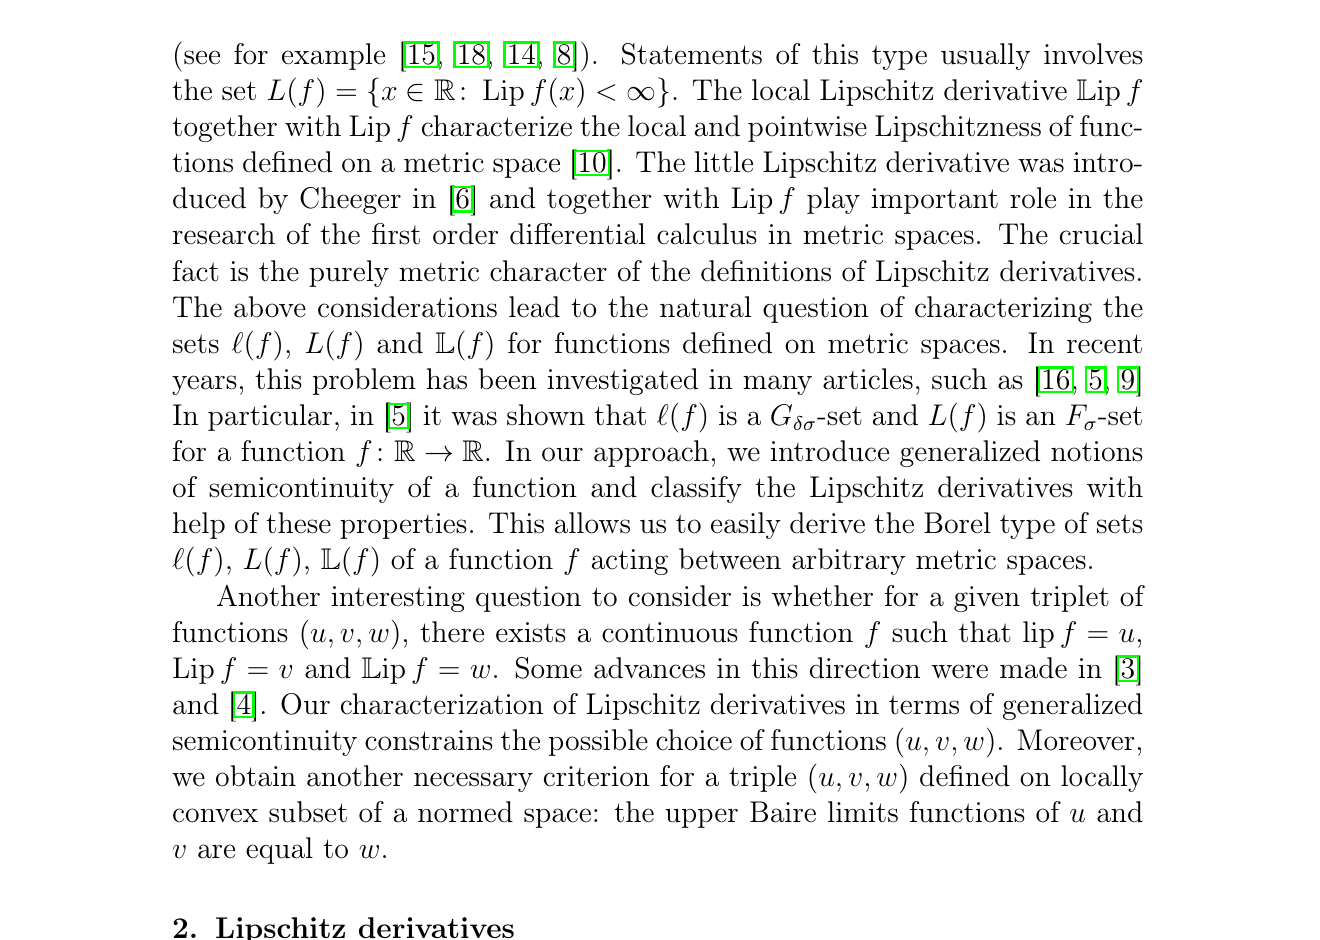
\includegraphics[width=0.96\linewidth]{figures/inverse_question_crop.png}
\end{center}

\noindent\textbf{Exact transcription.}
``Another interesting question to consider is whether for a given triplet of
functions $(u,v,w)$, there exists a continuous function $f$ such that
$\lipf f=u$, $\Lipf f=v$ and $\LLip f=w$.  Some advances in this direction
were made in [3] and [4].  Our characterization of Lipschitz derivatives in
terms of generalized semicontinuity constrains the possible choice of
functions $(u,v,w)$.  Moreover, we obtain another necessary criterion for a
triple $(u,v,w)$ defined on locally convex subset of a normed space: the upper
Baire limits functions of $u$ and $v$ are equal to $w$.''

For a function $g$ on a metric space, write
\[
 g^\vee(x)=\inf_{U\ni x}\sup_{y\in U}g(y)
\]
for its upper Baire function.  The cited necessary criterion is Theorem~7.1
on source PDF p.~16:

\begin{center}

\includegraphics[width=0.94\linewidth]{figures/source_theorem_crop.png}
\end{center}

\noindent\textbf{Exact transcription of Theorem 7.1.}
``Let $D$ be a locally convex subset of a normed space $X$ and let
$f:D\to\R$ be a function.  Then
\[
 (\lipf f)^\vee=(\Lipf f)^\vee=\LLip f.
\]''

We isolate the metric geometry behind this theorem and also test whether the
source's full list of necessary conditions could be sufficient for the
inverse problem.

\section{Definitions and proof intuition}

For a map $f:X\to Y$ between metric spaces, the three derivatives at $x$ are
\begin{align*}
 \lipf f(x)&=\liminf_{r\downarrow0}\frac1r
   \sup_{y\in B(x,r)}d_Y(f(y),f(x)),\\
 \Lipf f(x)&=\limsup_{y\to x}\frac{d_Y(f(y),f(x))}{d_X(y,x)},\\
 \LLip f(x)&=\limsup_{(y,z)\to(x,x)}
   \frac{d_Y(f(y),f(z))}{d_X(y,z)}.
\end{align*}
The source proves that $\lipf f$ is $\mathcal F_\sigma$-lower,
$\Lipf f$ is $\mathcal F_\sigma$-upper, and $\LLip f$ is upper
semicontinuous for continuous $f$.

\begin{definition}
Let $C\geq1$.  A metric space $X$ is \emph{asymptotically
$C$-quasiconvex at $x$} if, for every neighborhood $V$ of $x$ and every
$\eta>0$, there is a neighborhood $U\subseteq V$ of $x$ such that every
$y,z\in U$ can be joined by a rectifiable curve contained in $V$ of length
at most $(C+\eta)d_X(y,z)$.
\end{definition}

\subsection*{Proof Intuition}

Convexity in the source proof serves one purpose: it supplies a shortest
curve between nearby points.  Along an arc-length-parametrized curve $c$,
the little lip of $f\circ c$ is no larger than the little lip of $f$ on the
ambient space.  The one-dimensional rigidity theorem then integrates this
infinitesimal bound along $c$.  Short curves therefore convert the upper
Baire envelope of little lip into a bound for the local Lipschitz derivative.
Length spaces have curves arbitrarily close to shortest, so the distortion
factor tends to one.  Two branches that approach tangentially, however, can
have very small ambient separation but require a long detour; the local
derivative detects the cross-branch quotient while both pointwise derivatives
do not.

\section{A quantitative metric extension}

\begin{lemma}[Curve integration]\label{lem:curve}
Let $c:[0,L]\to X$ be parametrized by arc length and suppose
$\lipf f(c(t))\leq\gamma$ for all $t$.  Then
\[
 d_Y(f(c(0)),f(c(L)))\leq\gamma L.
\]
\end{lemma}

\begin{proof}
Since $c$ is $1$-Lipschitz,
\[
 \sup_{|s-t|<r}\frac{d_Y(f(c(s)),f(c(t)))}r
 \leq
 \sup_{d_X(y,c(t))<r}\frac{d_Y(f(y),f(c(t)))}r.
\]
Taking lower limits gives
$\lipf(f\circ c)(t)\leq\lipf f(c(t))\leq\gamma$.  The interval case of
Theorem~6.4 in the source gives the conclusion.  To see directly that its
real-valued interval estimate suffices for an arbitrary metric target, fix
$q\in Y$ and apply it to
$h_q(t)=d_Y(f(c(t)),q)$; then $\lipf h_q\leq\lipf(f\circ c)$.  Taking
$q=f(c(0))$ gives the displayed inequality.
\end{proof}

\begin{theorem}[Quantitative Baire-envelope bound]\label{thm:quant}
Suppose $X$ is asymptotically $C$-quasiconvex at $x$.  For every continuous
map $f:X\to Y$ into any metric space,
\begin{equation}
 (\lipf f)^\vee(x)\leq(\Lipf f)^\vee(x)\leq\LLip f(x)
 \leq C(\lipf f)^\vee(x).                                  \tag{1}
\end{equation}
\end{theorem}

\begin{proof}
The first two inequalities follow from
$\lipf f\leq\Lipf f\leq\LLip f$ and upper semicontinuity of $\LLip f$.
Put $A=(\lipf f)^\vee(x)$.  If $A=\infty$, there is nothing to prove.
Choose $\gamma>A$.  Some neighborhood $V$ of $x$ satisfies
$\lipf f<\gamma$ throughout $V$.  Given $\eta>0$, choose $U\subseteq V$
from asymptotic quasiconvexity.  Lemma~\ref{lem:curve} applied to the joining
curves gives
\[
 d_Y(f(y),f(z))\leq\gamma(C+\eta)d_X(y,z),\qquad y,z\in U.
\]
Thus $\LLip f(x)\leq\gamma(C+\eta)$.  Let first
$\gamma\downarrow A$ and then $\eta\downarrow0$.
\end{proof}

\begin{corollary}[Locally length domains]\label{cor:length}
If $X$ is locally a length space, then for every metric space $Y$ and every
continuous $f:X\to Y$,
\[
 (\lipf f)^\vee=(\Lipf f)^\vee=\LLip f.
\]
\end{corollary}

\begin{proof}
Fix $x$, a neighborhood $V$, and $\eta>0$.  Work in a length-space
neighborhood of $x$ and choose a small ball $B(x,R)\subseteq V$.  If
$y,z\in B(x,R/4)$, a curve of length at most
$(1+\min\{\eta,1/4\})d_X(y,z)$ remains in $B(x,R)$: its distance from $x$
is bounded by the distance from $x$ to $y$ plus the length already traversed.
Hence $X$ is asymptotically $1$-quasiconvex at $x$, and
Theorem~\ref{thm:quant} applies.
\end{proof}

This includes geodesic spaces, Riemannian and Finsler manifolds, metric
graphs, CAT spaces, and open subsets of length spaces.  It also allows
arbitrary metric codomains, whereas source Theorem~7.1 is stated for
real-valued maps.

\section{Two obstructions for the inverse problem}

\begin{proposition}[The source conditions are not sufficient]\label{prop:spike}
On $I=[-1,1]$, let
\[
 u=v=w=\mathbf1_{\{0\}}.
\]
This triple satisfies $u\leq v\leq w$, the source's respective
$\mathcal F_\sigma$-lower, $\mathcal F_\sigma$-upper, and upper
semicontinuity conditions, and $u^\vee=v^\vee=w$.  Nevertheless, no
continuous $f:I\to\R$ realizes
$(u,v,w)=(\lipf f,\Lipf f,\LLip f)$.
\end{proposition}

\begin{proof}
The singleton is closed, its complement is open (hence $F_\sigma$ in a
metric space), and $w$ is upper semicontinuous; these observations verify
all the stated regularity and envelope conditions.

If such $f$ existed, then $\lipf f\leq1$.  The interval case of source
Theorem~6.4 would make $f$ $1$-Lipschitz, hence absolutely continuous and
differentiable almost everywhere.  At every differentiability point
$x\ne0$, source Theorem~3.2 gives
$|f'(x)|=\Lipf f(x)=0$.  Thus $f'=0$ almost everywhere, so $f$ is constant.
Its three Lipschitz derivatives are then zero at the origin, a contradiction.
\end{proof}

\begin{theorem}[Tangential double-arc counterexample]\label{thm:cusp}
For every $\alpha>1$, set
\[
 X_\alpha=\{(t,t^\alpha),(t,-t^\alpha):0\leq t\leq1\}
 \subset\R^2
\]
with the Euclidean subspace metric, let $o=(0,0)$, and let $f(x,y)=y$.
Then $X_\alpha$ is compact and connected, while
\[
 (\lipf f)^\vee(o)=(\Lipf f)^\vee(o)=0,
 \qquad \LLip f(o)=1.                                      \tag{2}
\]
\end{theorem}

\begin{proof}
The coordinate projection $f$ is globally $1$-Lipschitz.  At the origin,
the pointwise quotient along either branch is
\[
 \frac{t^\alpha}{\sqrt{t^2+t^{2\alpha}}}\longrightarrow0,
\]
so $\lipf f(o)=\Lipf f(o)=0$.  At a nonzero point of either smooth branch,
all pointwise derivatives equal the norm of the vertical coordinate on the
unit tangent,
\[
 m_\alpha(t)=\frac{\alpha t^{\alpha-1}}
 {\sqrt{1+\alpha^2t^{2\alpha-2}}}\longrightarrow0
 \qquad(t\downarrow0).
\]
This proves both upper-envelope equalities in (2).

For the opposite points $y_t=(t,t^\alpha)$ and
$z_t=(t,-t^\alpha)$,
\[
 \frac{|f(y_t)-f(z_t)|}{\|y_t-z_t\|_2}
 =\frac{2t^\alpha}{2t^\alpha}=1.
\]
They converge to $o$, so $\LLip f(o)\geq1$; global $1$-Lipschitzness gives
the reverse inequality.  Thus (2) holds.
\end{proof}

The failure is exactly a path-distortion phenomenon.  Every path in
$X_\alpha$ joining $y_t$ to $z_t$ passes through $o$, so its length is at
least $2t$, whereas the ambient distance is $2t^\alpha$.  Their ratio
$t^{1-\alpha}$ diverges.

\section{Verification, limitations, and novelty}

The accompanying verifier evaluates the radial quotient, the exact tangent
slope, the cross-branch quotient, and the path/chord distortion for
$\alpha=3/2,2,3$ down to $t=10^{-9}$.  It independently compares the tangent
formula with centered finite differences.  Every check passed; the largest
finite-difference error was below $2.6\cdot10^{-11}$.

\textbf{Scope limitation.}  Proposition~\ref{prop:spike} rules out the
obvious sufficiency conjecture, and Corollary~\ref{cor:length} resolves the
domain-geometry component of the strongest joint constraint.  The full
inverse problem remains open: even on an interval, realizability includes
additional measure-theoretic and integrability constraints not captured by
this argument.

\textbf{Bounded novelty audit.}  The run indexes and primary-source arXiv
searches through 13 August 2026 were checked using arXiv:2509.20849 and the
phrases ``little Lipschitz derivative,'' ``upper Baire,'' ``length space,''
and ``lower scaled oscillation.''  Searches found the source,
arXiv:1910.14527, and recent Takagi--van der Waerden constructions, but no
locally length extension, quantitative quasiconvex bound, singleton-spike
obstruction, or tangential-double-arc example.  Novelty is plausible, not
certified.

\textbf{Human-review recommendation:} send to a metric-analysis expert.  The
highest-value checks are the metric-codomain scalarization in
Lemma~\ref{lem:curve}, the neighborhood bookkeeping in
Corollary~\ref{cor:length}, and the assertion that the singleton indicator
meets the source's generalized semicontinuity definitions.

\begin{thebibliography}{9}
\bibitem{MW}
O.~V. Maslyuchenko and Z.~M. W\'ojcicki,
\emph{Classification of Lipschitz derivatives in terms of semicontinuity and
the Baire limit functions}, arXiv:2509.20849 (2025).

\end{thebibliography}

\end{document}
